\documentclass{article}

\usepackage{tikz}
\usetikzlibrary{automata, positioning, arrows}

\author{Nikita Servais}
\title{Assignment 2: MVC using Scala Play}
\date{January 7, 2023}

\begin{document}
    \maketitle


    \section{Introduction}
    This report describes the design and implementation of a social media application using the Scala Play framework.
    The application is a simple social media application that allows users to post a picture with a description, like post, comment on post and see other users post.
    The application is implemented using the Model-View-Controller (MVC) design pattern and the play framework using scala.
    The models represent the data and the business logic of the application.
    The controllers handle the user requests and update the models.
    The views present the data to the users.


    \section{Models}
    The application has three main models: \textbf{User}, \textbf{Post}, and \textbf{Comment}.

    The \textbf{User} model represents the users of the application.
    It consists of a username and a password.
    For security reasons, it would be advisable to implementing a hash for the password before storing it.

    The \textbf{Post} model represents the posts that users create and share on the platform.
    Each post has an ID, the username of the user who posted it, the file path to the image of the post, the date of creation, a description, a list of likes, and a list of comments.


    The \textbf{Comment} model represents the comments that users leave on posts.
    Each comment has the username of the user who commented and the content of the comment.

    A Data Access Object (DAO) layer is used to interface with the database.
    This is used to retrieve and store the objects in the database.
    In this case, there is no database, so the objects are stored in memory.


    \section{Controllers}
    The application has a controller for each corresponding to a view.
    There is also a \textbf{HomeController} that redirects to the feed and can log out the user.
    Each controller has an index method to show the view of the page.
    For each possible action on the page, there is a method to manage that action.
    For example, the \textbf{FeedController} has a method to handle like a post by the user.
    It will retrieve the post from the database, add the user to the list of likes, and update the post in the database (this is done by reference, as there is no database).


    \section{Views}
    The views of the application are represented by HTML templates.
    This make use of the templating engine of the Play framework.
    These templates are rendered by the controllers and presented to the users.
    The views include a registration page, a login page, a feed page, a profile page, an upload page, and a post page.


    \section{Diagram}
    The diagram in Figure \ref{fig:state-machine} in the report illustrates the flow of the application.
    The nodes represent the different pages (views) of the application, and the arrows represent the actions that a user can take to navigate from one page to another.

    \begin{figure}[ht]
        \centering
        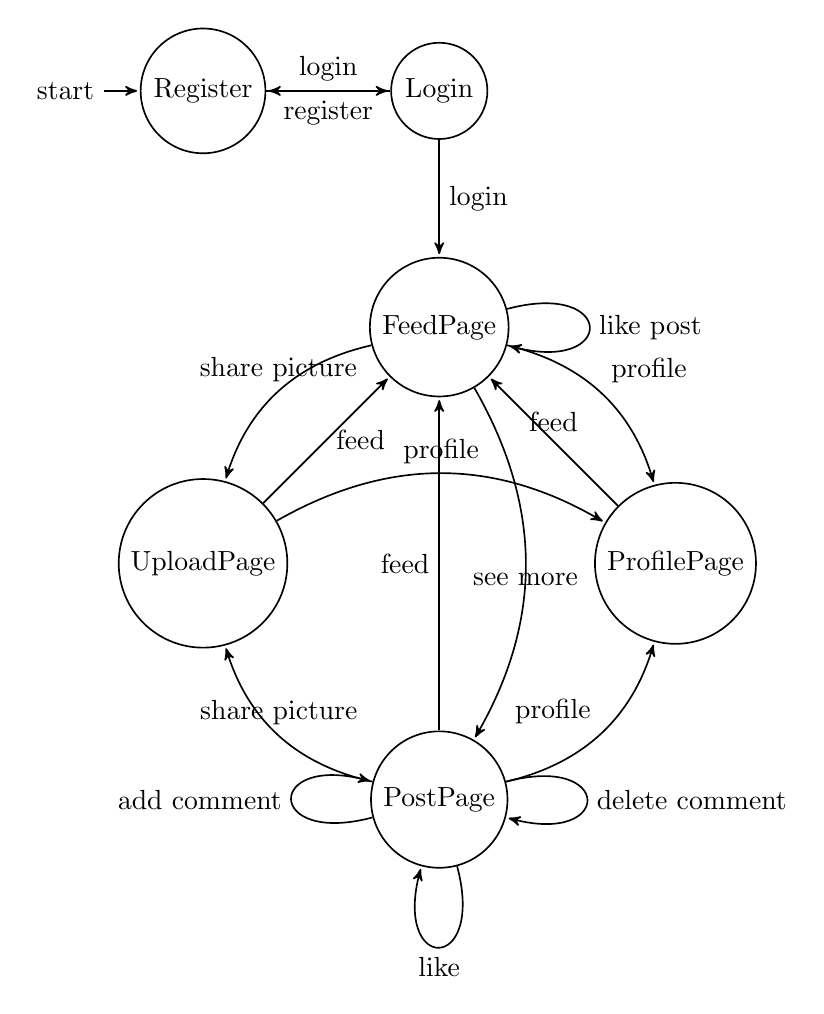
\begin{tikzpicture}[->,>=stealth',shorten >=1pt,auto,node distance=3cm,
            semithick]
            \tikzstyle{every state}=[]

            \node[initial,state] (R)                    {Register};
            \node[state]         (L) [right of=R]       {Login};
            \node[state]         (F) [below of=L]       {FeedPage};
            \node[state]         (PV) [right of=F, below of=F]      {ProfilePage};
            \node[state]         (U) [left of=F, below of=F]       {UploadPage};
            \node[state]         (P) [left of=PV, below of=PV]       {PostPage};

            \path (R) edge node {login} (L)
            (L) edge node {register} (R)
            (L) edge node {login} (F)

            (F) edge  [loop right]            node {like post} (F)
            (F) edge  [bend left, below]         node {see more} (P)
            (F) edge [bend right, above]  node {share picture} (U)
            (F) edge [bend left] node {profile} (PV)

            (U) edge [bend left] node {profile} (PV)
            (U) edge    [right]          node {feed} (F)

            (PV) edge  [above]           node {feed} (F)
            (P) edge node {feed} (F)
            (P) edge [loop below] node {like} (P)
            (P) edge [loop left]  node {add comment} (P)
            (P) edge [loop right] node {delete comment} (P)
            (P) edge [bend left, above] node {share picture} (U)
            (P) edge [bend right] node {profile} (PV);

        \end{tikzpicture}
        \caption{State machine of the event flow of the application}
        \label{fig:state-machine}
    \end{figure}
\end{document}
